\chapter{GIỚI THIỆU MẠNG HỌC SÂU ỨNG DỤNG TRONG PHÂN VÙNG ẢNH}
\section{Giới thiệu về mạng học sâu U-net}

\begin{figure}[h]
	\centering
	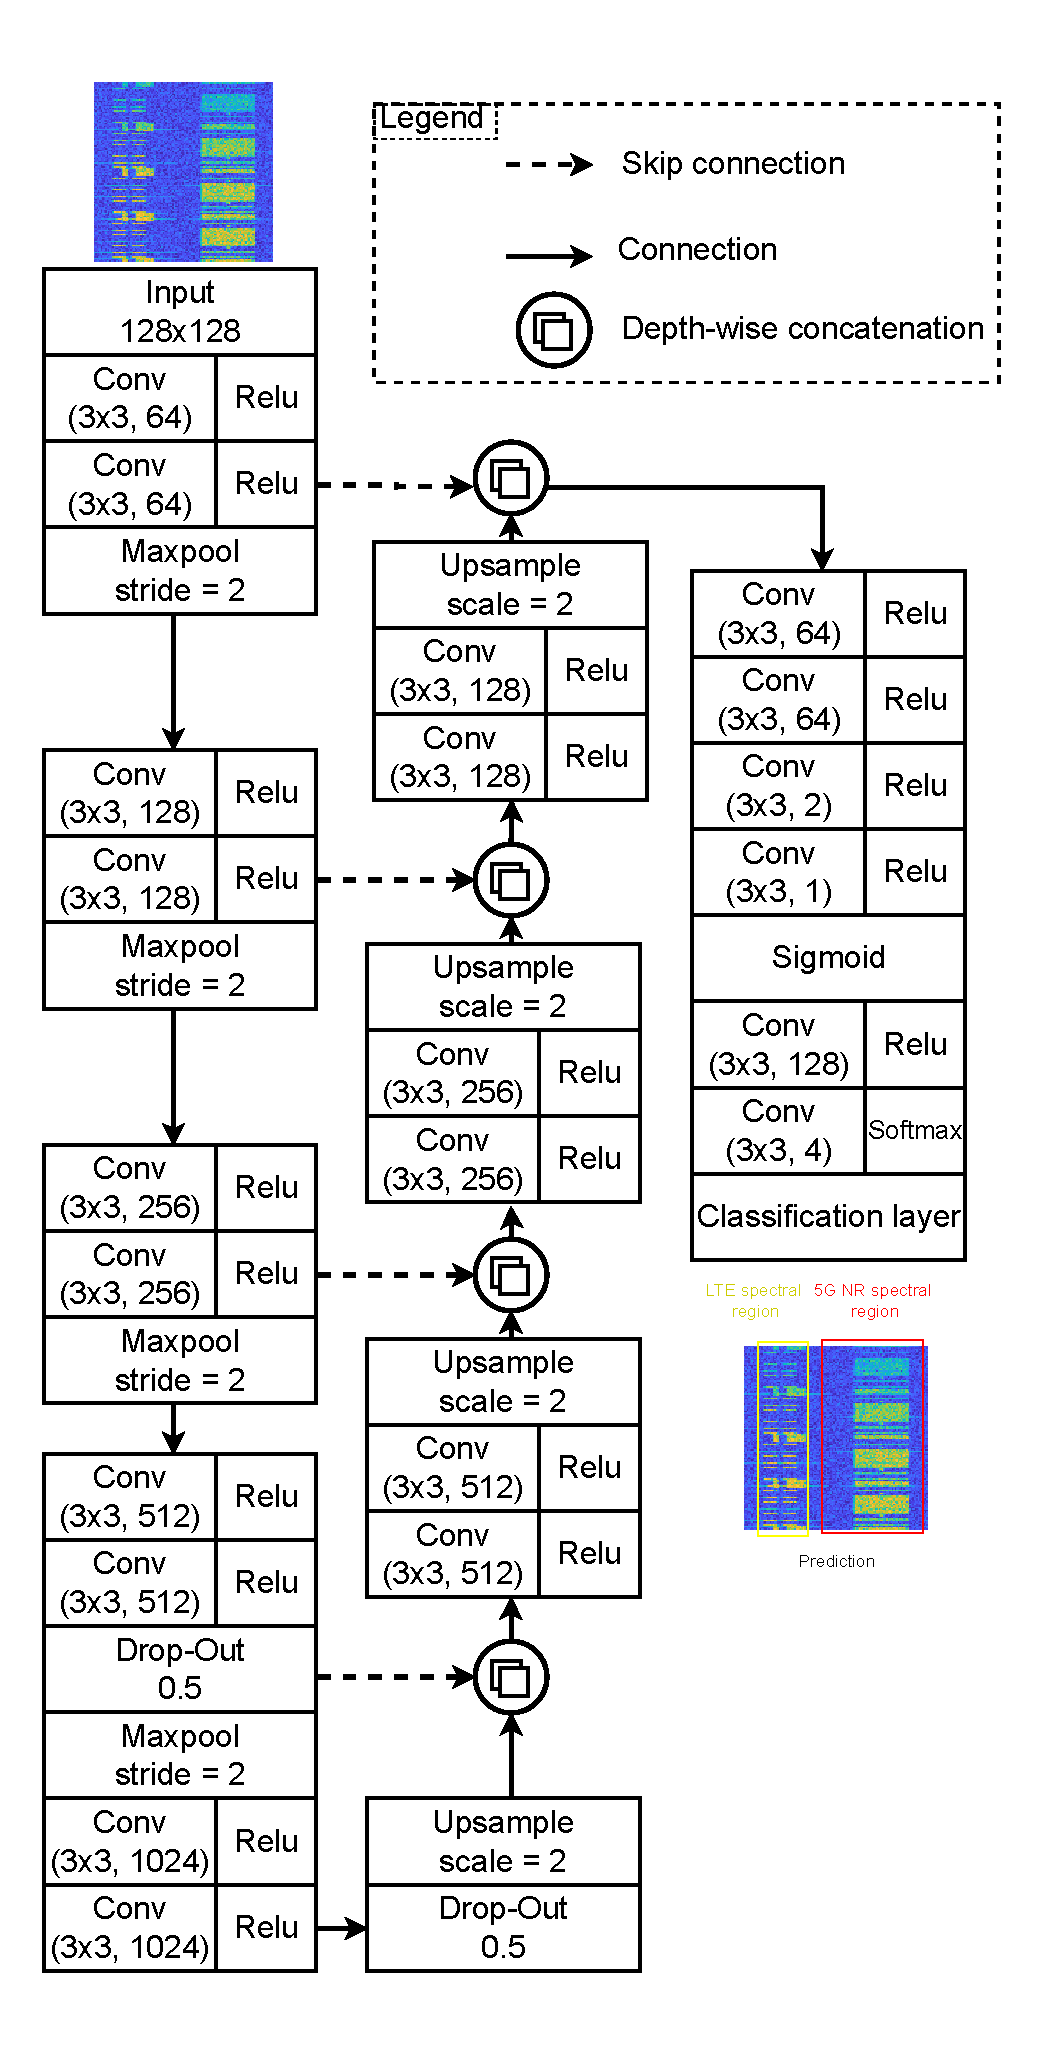
\includegraphics[width=80mm]{fig/Design-Unet.pdf}
        \captionsetup{justification=centering}
	\caption{Kiến trúc mạng U-net.}
	\label{fig_U-net}
\end{figure}

Mô hình mạng U-net được giới thiệu bởi tác giả Ronneberger \cite{aghalari2021brain} cùng với các cộng sự nhằm ứng dụng vào lĩnh vực nhận diện và phân loại ảnh chụp quang học. U-net là một mô hình mạng nơ-ron tích chập toàn phần đã được cải tiến và phát triển dựa trên cấu trúc của mạng tích chập truyền thống. Đặc trưng của U-net là cấu trúc đối xứng hình chữ "U", được minh họa ở Hình \ref{fig_U-net}. Phần mã hóa của mạng U-net tương tự như các mạng tích chập khác, bao gồm các lớp tích chập và tổng hợp tối đa để trích xuất đặc trưng từ ảnh. Trong Hình \ref{fig_U-net}, các lớp tích chập sử dụng cửa sổ trượt kích thước $3\times3$, và các lớp tổng hợp tối đa sử dụng cửa sổ trượt kích thước $2\times2$, giảm kích thước đầu vào đi một nửa cả về chiều dài và chiều rộng.

Thông qua các lần lặp của tích chập và tổng hợp tối đa, kích thước của ảnh sẽ giảm dần, tăng cường sự phức tạp của các đặc trưng được học. Để đảm bảo rằng thông tin chiều sâu đủ đáng kể, việc tăng số lớp tích chập ở cuối phần mã hóa là rất quan trọng để cải thiện hiệu suất học.

Một điểm đặc biệt của U-net là cấu trúc đối xứng của phần mã hóa và giải mã. Trong phần giải mã, việc mở rộng kích thước của ảnh tương đương với việc giảm kích thước của ảnh trong phần mã hóa tương ứng. Ngoài việc mở rộng kích thước, các lớp trong phần giải mã còn được kết nối đối xứng với các lớp tương ứng trong phần mã hóa, giúp khôi phục lại thông tin bị mất trong quá trình tổng hợp. Sau mỗi lần mở rộng trong phần giải mã, kết quả được kết hợp với kết quả của lớp giảm kích thước tương ứng trong phần mã hóa, trước khi đi qua các lớp tích chập và tiếp tục quá trình mở rộng.

\section{Mô hình mạng SegNet}

\begin{figure}[h]
	\centering
	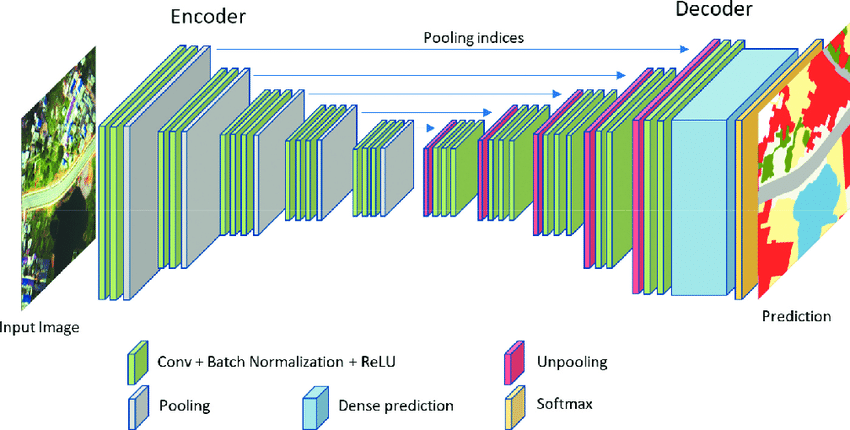
\includegraphics[width=120mm]{fig/SegNet-architecture.png}
        \captionsetup{justification=centering}
	\caption{Kiến trúc mạng SegNet (nguồn Internet).}
	\label{fig_SegNet}
\end{figure}

SegNet là một mô hình mạng nơ-ron tích chập được công bố bởi tác giả Badrinarayanan và các cộng sự~\cite{badrinarayanan2017segnet}, đặc biệt được thiết kế để giải quyết bài toán phân đoạn ảnh. Mô hình này có nhiều điểm tương đồng với U-net, bao gồm một phần mã hóa được xây dựng theo kiến trúc mạng tích chập thông thường, với các lớp tích chập và tổng hợp được lấy cảm hứng từ các mô hình nổi tiếng như VGG16, VGG19 và ResNet. Tuy nhiên, SegNet loại bỏ lớp kết nối đầy đủ ở cuối của mạng.

Như được minh họa trong Hình \ref{fig_SegNet}, phần mã hóa của SegNet sử dụng cấu trúc của mạng VGG16, bao gồm 13 lớp tích chập và 5 lớp giảm kích thước. Phần giải mã của SegNet cũng bao gồm các lớp mở rộng và tích chập, nhưng điểm đặc biệt và làm nên hiệu quả của mô hình nằm ở các lớp mở rộng.

Trong SegNet, đầu ra của các lớp mở rộng được mở rộng dựa trên vị trí ban đầu của các pixel tương ứng ở các lớp giảm kích thước trước đó. Để thực hiện điều này, vị trí của các pixel lớn nhất ở đầu vào của các lớp giảm kích thước được lưu giữ lại. Khi đi qua các lớp tích chập, các pixel đầu ra của lớp giảm kích thước sẽ được đưa về vị trí ban đầu của chúng trước khi thực hiện giảm kích thước.

So với U-net, SegNet không có các kết nối với các biểu đồ đặc trưng của các lớp trước, nhưng thay vào đó, thông tin quan trọng được lưu trữ và chuyển tiếp tới các lớp sau là vị trí của các pixel. Điều này làm cho SegNet tiêu tốn ít bộ nhớ hơn trong các ứng dụng và thiết bị nhúng. Với phần giải mã phức tạp và lớn với nhiều tầng tích chập, SegNet đã cho thấy kết quả khả quan trong nhiều thử nghiệm thực tế.

\section{Mô hình mạng SqueezeSegV2}

\begin{figure}[h]
	\centering
	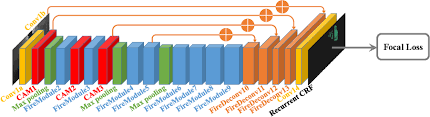
\includegraphics[width=120mm]{fig/SegNetV2-architecture.png}
        \captionsetup{justification=centering}
	\caption{Kiến trúc mạng SqueezeSegV2 (nguồn Internet).}
	\label{fig_SegNet}
\end{figure}

SqueezeSegV2~\cite{wu2019squeezesegv2}, là một mạng nơ-ron tích chập được phát triển dựa trên mô hình giải mã - mã hóa, đặc biệt thiết kế để phân loại dữ liệu điểm thu thập từ LiDAR trong ứng dụng phân vùng ngữ nghĩa. Đây là phiên bản nâng cấp của mô hình gốc có tên là SqueezeSeg. SqueezeSeg được tạo ra để phát hiện và phân loại các đối tượng quan trọng trong không gian 3D bằng cách biểu diễn phân vùng ngữ nghĩa 3D dưới dạng phân loại cho từng điểm dữ liệu. Dữ liệu điểm từ LiDAR được chuyển đổi thành hình ảnh 2D thông qua cơ chế phóng chiếu hình cầu, tạo nên một sự cân đối giữa độ chính xác và độ phức tạp.

Kiến trúc của SqueezeSeg được xây dựng bằng cách sử dụng các mô-đun Fire và mô-đun Deconvolution (Deconv), nhằm khắc phục việc mất mát thông tin chi tiết ở mức thấp do các phép giảm kích thước dữ liệu. Đặc biệt, SqueezeSegV2 cải tiến bằng việc giới thiệu một mô-đun tổng hợp ngữ cảnh mới (CAM) để giảm thiểu tác động tiêu cực của nhiễu dropout trong dữ liệu LiDAR, cũng như sử dụng hàm mất mát trọng tâm (focal loss) thay thế cho hàm mất mát cross-entropy ban đầu. Hàm mất mát trọng tâm giải quyết vấn đề mất cân bằng lớp bằng cách nhấn mạnh các mẫu âm trong quá trình huấn luyện.

So với U-net, SqueezeSegV2 tập trung vào việc phân loại dữ liệu điểm từ LiDAR thay vì phân đoạn hình ảnh. Điều này làm cho SqueezeSegV2 phù hợp hơn trong các ứng dụng cụ thể như tự lái xe, nơi mà dữ liệu LiDAR là quan trọng. SqueezeSegV2 cũng có một kiến trúc mạng phức tạp và các cải tiến trong hàm mất mát, giúp cải thiện độ chính xác và hiệu suất của mô hình. Tuy nhiên, U-net vẫn được ưa chuộng trong các ứng dụng phân đoạn hình ảnh chung do tính linh hoạt và khả năng áp dụng rộng rãi của nó.

\section{Đánh giá ưu và nhược điểm}
U-Net, SegNet và SqueezeSegV2 là ba mô hình quan trọng trong lĩnh vực phân vùng ngữ nghĩa ảnh, mỗi một trong số chúng đều có những đặc điểm và ưu điểm riêng.

U-Net nổi tiếng với cấu trúc đối xứng hình chữ "U", giúp nó trích xuất và tái tạo các đặc trưng cục bộ và toàn cục từ ảnh. Kiến trúc của U-Net giúp nó phù hợp với các tác vụ phân đoạn hình ảnh và đã được chứng minh hiệu quả trong nhiều ứng dụng y tế và địa lý. Tuy nhiên, U-Net có thể gặp khó khăn trong việc xử lý các đối tượng lớn và trong môi trường có nhiều nhiễu.

SegNet, trên cơ sở của mô hình tích chập truyền thống như VGG16 hoặc VGG19, chú trọng vào việc tái tạo vị trí của các pixel thông qua các lớp mở rộng và tích chập. Điều này giúp giữ lại thông tin về vị trí, đặc biệt quan trọng trong các ứng dụng nhúng và y tế. SegNet cũng có khả năng xử lý tốt các đối tượng lớn và nhiều nhiễu hơn so với U-Net.

SqueezeSegV2 là một mô hình tập trung vào việc phân loại dữ liệu điểm từ LiDAR, thích hợp cho các ứng dụng tự lái xe. Với cải tiến trong kiến trúc mạng và hàm mất mát, SqueezeSegV2 giúp cải thiện độ chính xác và hiệu suất trong việc phân loại các đối tượng trong không gian 3D từ dữ liệu LiDAR.

\section{Tệp dữ liệu khảo sát}
\begin{figure}[!h]
    \centering
    \footnotesize
    \begin{tabular}{ccccccc}
        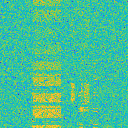
\includegraphics[width=0.12\textwidth]{fig/LTE_NR_0db.png} & 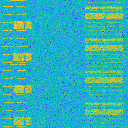
\includegraphics[width=0.12\textwidth]{fig/LTE_NR_5db.png} &
        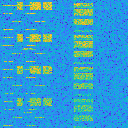
\includegraphics[width=0.12\textwidth]{fig/LTE_NR_10db.png}&
        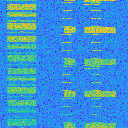
\includegraphics[width=0.12\textwidth]{fig/LTE_NR_15db.png}& 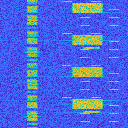
\includegraphics[width=0.12\textwidth]{fig/LTE_NR_20db.png}&
        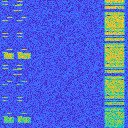
\includegraphics[width=0.12\textwidth]{fig/LTE_NR_25db.png}&
        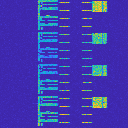
\includegraphics[width=0.12\textwidth]{fig/LTE_NR_30db.png}
        \\
        (a) & (b) & (c) & (d) & (e) & (f) & (g)
    \end{tabular}
    \caption{Dữ liệu giao thoa phổ 5G NR và LTE với SNR khác nhau: (a) 0 dB, (b) 5 dB, (c) 10 dB, (d) 15 dB, (e) 20 dB, (f) 25 dB, (g) 30 dB.}
    \label{fig_dataset5GLTE}
\end{figure}

\begin{figure}[!h]
    \centering
    \footnotesize
    \begin{tabular}{ccccccc}
        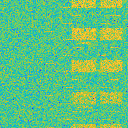
\includegraphics[width=0.12\textwidth]{fig/NR_frame_0db.png} & 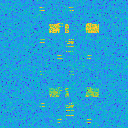
\includegraphics[width=0.12\textwidth]{fig/NR_frame_5db.png} &
        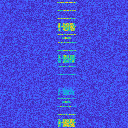
\includegraphics[width=0.12\textwidth]{fig/NR_frame_10db.png} &
        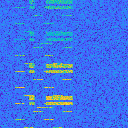
\includegraphics[width=0.12\textwidth]{fig/NR_frame_15db.png} & 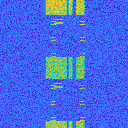
\includegraphics[width=0.12\textwidth]{fig/NR_frame_20db.png} &
        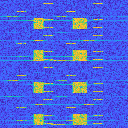
\includegraphics[width=0.12\textwidth]{fig/NR_frame_25db.png} &
        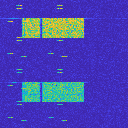
\includegraphics[width=0.12\textwidth]{fig/NR_frame_30db.png}
        \\
        (a) & (b) & (c) & (d) & (e) & (f) & (g)
    \end{tabular}
    \caption{Dữ liệu phổ 5G với SNR khác nhau: (a) 0 dB, (b) 5 dB, (c) 10 dB, (d) 15 dB, (e) 20 dB, (f) 25 dB, (g) 30 dB.}
    \label{fig_dataset5G}
\end{figure}

\begin{figure}[!h]
    \centering
    \footnotesize
    \begin{tabular}{ccccccc}
        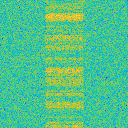
\includegraphics[width=0.12\textwidth]{fig/LTE_frame_0db.png} & 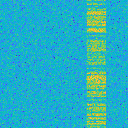
\includegraphics[width=0.12\textwidth]{fig/LTE_frame_5db.png} &
        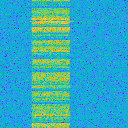
\includegraphics[width=0.12\textwidth]{fig/LTE_frame_10db.png} &
        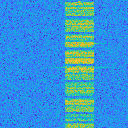
\includegraphics[width=0.12\textwidth]{fig/LTE_frame_15db.png} & 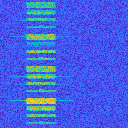
\includegraphics[width=0.12\textwidth]{fig/LTE_frame_20db.png} &
        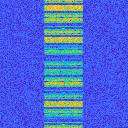
\includegraphics[width=0.12\textwidth]{fig/LTE_frame_25db.png} &
        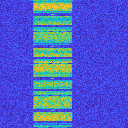
\includegraphics[width=0.12\textwidth]{fig/LTE_frame_30db.png}
        \\
        (a) & (b) & (c) & (d) & (e) & (f) & (g)
    \end{tabular}
    \caption{Dữ liệu phổ LTE với SNR khác nhau: (a) 0 dB, (b) 5 dB, (c) 10 dB, (d) 15 dB, (e) 20 dB, (f) 25 dB, (g) 30 dB.}
    \label{fig_datasetLTE}
\end{figure}

\begin{table}[h]
\centering
\caption{Thông tin về dữ liệu đầu vào cho mỗi phân loại}
\label{tab2}
\begin{tabular}{c|c|c|c}
\hline
\hline
\multicolumn{4}{c}{\textbf{Dataset Information}} \\
\hline
\textbf{Category} & \textbf{No.Samples} & \textbf{Image size} & \textbf{SNR (dB)}\\
\hline
\hline
LTE         & $5,000$ & $128 \times 128$ & $[0, 30]$ \\
5G          & $5,000$ & $128 \times 128$ & $[0, 30]$ \\
5G and LTE  & $5,000$ & $128 \times 128$ & $[0, 30]$ \\
\hline
\hline
\end{tabular}
\end{table}

Trong dự án nghiên cứu này, chúng tôi đã phải đối mặt với những thách thức thực tế, từ việc quản lý chi phí cho đến bảo vệ quyền riêng tư. Để nắm bắt bức tranh toàn diện về mạng 5G và LTE, chúng tôi đã sử dụng bộ công cụ 5G trong Matlab để tạo ra một tập dữ liệu phổ tổng hợp, bao gồm ba loại chính: 5G, LTE và các khung giao thoa giữa 5G và LTE.

Tập dữ liệu của chúng tôi bao gồm tổng cộng 5,000 mẫu cho mỗi loại, mỗi mẫu có kích thước hình ảnh là $128 \times 128$. Đặc biệt, chúng tôi đã khám phá một loạt các mức độ tín hiệu tạp âm-tỷ lệ tín hiệu (SNR) từ $0$ đến $30$ dB, để mô phỏng các tình huống khác nhau trong môi trường thực tế.


\section{Kết luận}
Trong đề tài này, học viên đã đề suất đề tài liên quan dến giám sát phổ tín hiệu dựa trên các mô hình học sâu, nhằm mục đích phát hiện các dải băng tần chưa được sử dụng và cấp phát cho các loại sóng di động cũng như ra-da khác. Dựa trên sự so sánh giữa các mô hình học sâu và những kinh nghiệm đã được tích lũy từ những đề tài nghiên cứu trước đó, học viên quyết định chọn mô hình U-net để tiếp tục tìm hiểu chi tiết và tìm ra giải pháp tăng cường hiệu năng của mô hình học sâu U-net sao cho đáp ứng được nhu cầu thực tế của đề tài. Việc lựa chọn U-Net cho việc cảm biến phổ có nhiều ưu điểm quan trọng:

\begin{itemize}
    \item \textbf{Xử lý hình ảnh 2D:} U-Net được thiết kế đặc biệt cho việc phân đoạn hình ảnh, phù hợp cho dữ liệu từ cảm biến phổ trong không gian 2D.
    \item \textbf{Kiến trúc đặc biệt:} Kiến trúc đối xứng hình chữ "U" của U-Net giúp nó trích xuất đặc trưng cục bộ và toàn cục từ ảnh một cách hiệu quả. Điều này rất hữu ích trong việc xử lý dữ liệu từ cảm biến phổ, nơi mà việc trích xuất các đặc trưng quan trọng từ dữ liệu là cần thiết.
    \item \textbf{Độ linh hoạt:} U-Net có thể dễ dàng được điều chỉnh và tinh chỉnh cho các yêu cầu cụ thể của ứng dụng cảm biến phổ. Cấu trúc mạng linh hoạt và khả năng đào tạo hiệu quả giúp nó thích hợp cho nhiều loại dữ liệu và nhiều tác vụ khác nhau.
    \item \textbf{Hiệu suất và hiệu quả:} U-Net đã được chứng minh hiệu quả trong nhiều ứng dụng phân đoạn hình ảnh, bao gồm cả việc xử lý dữ liệu từ cảm biến phổ. Với khả năng học và trích xuất đặc trưng tốt, U-Net có thể giúp tăng cường hiệu suất của hệ thống cảm biến phổ và giảm thiểu sai số.
    \item \textbf{Sử dụng trong các ứng dụng thực tế:} U-Net đã được sử dụng rộng rãi trong nhiều lĩnh vực, từ y tế đến xe tự lái và nông nghiệp. Sự phổ biến và khả năng thích nghi của nó làm cho U-Net trở thành một lựa chọn hợp lý cho việc xử lý dữ liệu từ cảm biến phổ trong các ứng dụng thực tế.
\end{itemize}



